\documentclass[12pt,letterpaper]{article}
%\documentstyle[11pt]{article}
\usepackage[utf8]{inputenc}
\usepackage{amsmath}
\usepackage{xfrac}
\usepackage{amsfonts}
\usepackage{amssymb}
\usepackage[version = 3]{mhchem}
\usepackage{chemstyle}
%%For Table perhaps%%
%\usepackage{graphics}
\usepackage{graphicx}
\usepackage{epstopdf}
%\usepackage{tabularx,ragged2e,booktabs,caption}
%\newcolumntype{C}[1]{>{\Centering}m{#1}}
%\renewcommand\tabularxcolumn[1]{C{#1}}
\usepackage[left=2cm,right=2cm,top=0.5cm,bottom=2cm]{geometry}
\usepackage{subcaption} 
\usepackage{caption}
\usepackage[colorlinks]{hyperref}
\usepackage[svgnames]{xcolor}
\hypersetup{citecolor=DeepPink4}
\hypersetup{linkcolor=DarkRed}
\hypersetup{urlcolor=DarkBlue}
\usepackage{cleveref}

\begin{document}
\setlength{\parindent}{0cm} 


\frenchspacing


\title {\Large{\textbf{Quiz 3---Water Treatment Processes}}\\ \large{CENG 340--Introduction to Environmental Engineering\\
Instructor: Deborah Sills\\ \textbf{18 October, 2013}}}
\author {}
\date {}
\maketitle

\vspace{-0.2 in}
\textbf{\large{Name:}}\\

\begin{enumerate}

\item \emph{(6 points)} Add labels to the following schematic of a drinking water treatment plant designed to treat surface water.  Labels should describe (in one or two words) the appropriate unit process.

\vspace{0.4in}

\begin{figure}
\centering
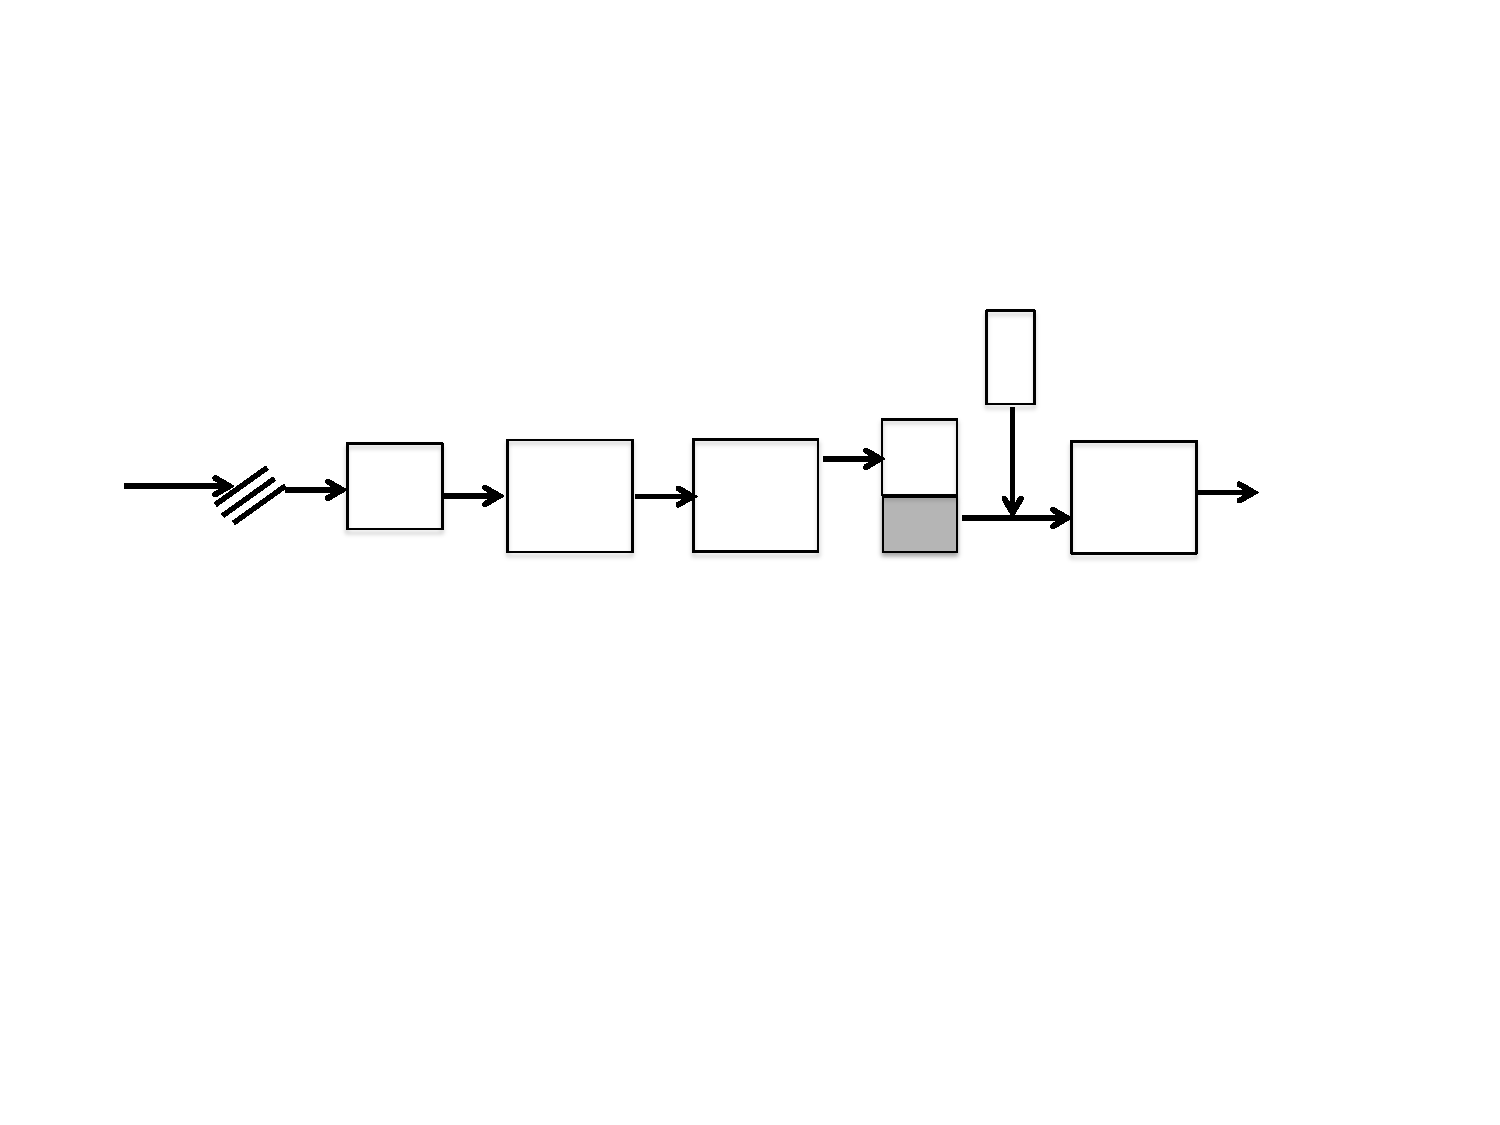
\includegraphics[width=1\textwidth]{surface}
\end{figure}

\vspace{0.7in}

\item Multiple Choice: one or more answers may be correct in each of the following questions.

\begin{enumerate}

\item \emph{(2 points)} The coagulation process
\begin{enumerate}
\item removes particles from water
\item neutralizes charged particles in water
\item filters particles in water
\item precipitates particles in water
\item requires slow mixing
\item requires rapid mixing
\end{enumerate} 

\vspace{0.1in}

\item \emph{(2 points)} Alum addition results in a reaction that 
\begin{enumerate}
\item consumes alkalinity
\item produces alkalinity
\item may require addition of alkalinity
\item operates best at pH between 7.7 to 9.9
\end{enumerate}



\end{enumerate}


\end{enumerate}





\end{document}